\section{Simulation homogener Plattenkondensator}\label{sec:ag3_3}
In dieser Aufgabe wird ein harmonischer Plattenkondensator in dem Simulationsprogramm \glqq FEMM \grqq{} nachgebaut. FEMM steht kostenfrei zur Verfügung und kann in Octave eingebunden werden.\\
Zunächst soll der Einfluss unterschiedlicher Randbedingungen auf das elektrische Feld eines Kondensators betrachtet werden. \\
Ein Kondensator ist eine Anordnung von zwei beliebigen Elektroden, die durch ein Dielektrikum von einander getrennt sind und die gleiche Ladung, aber mit unterschiedlicher Polarität in sich tragen, die Kapazität lässt sich mit $ C = \epsilon_{0}\epsilon_{r}\frac{A}{d}$ berechnen, wobei $A$ die Fläche der Platten, $d$ den Abstand der Platten, $\epsilon_{0}$ die elektrische Feldkonstante und $\epsilon_{r}$ die relative Permittivität des Dielektrikums beschreibt. Außerdem kann die Formel $C = \frac{Q}{U}$ zur Berechnung der Kapazität benutzt werden, $Q$ ist die Ladung in \si{\farad} und $U$ die Spannung in \SI{}{\volt}. \\ \\
Zum Bau des Kondensators werden in FEMM vier Punkte gesetzt und diese zu Linien verbunden. Der Abstand der Punkte beträgt sowohl in x-, als auch in y-Richtung \SI{30}{\centi\meter}. Genau genommen wird ein Quader erstellt, da die Kondensatorplatten quadratisch sein sollen, hat der Quader eine Tiefe von \SI{30}{\centi\meter}, jedoch verfügt FEMM nur eine 2-Dimensionale graphische Darstellung.\\
 Die linke und rechte Linie in Abbildung \ref{fig:kleinRand} stellen die beiden Kondensatorplatten dar, die obere und untere Linie dienen zur Berandung des elektrischen Felds. An der linken Platte des Kondensators liegt eine Spannung von \SI{1}{\volt} an, an der rechten Seite eine Spannung von \SI{0}{\volt}. Des Weiteren wurde in Abbildung \ref{fig:KäfigRand} ein Kondensator betrachtet, der nicht direkt, sondern durch einen äußeren Käfig berandet wird. Die inneren Linien markieren die beiden Kondensatorplatten, hier liegen die selben Spannungen wie im Vergleichsbild an.
\begin{figure}[h]
	\begin{subfigure}[c]{0.2\textwidth}
		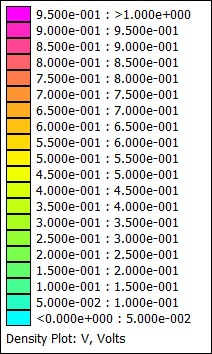
\includegraphics[width=\textwidth]{data/Skala}
		\caption{Skala}
		\label{fig:Skala}
	\end{subfigure}
	\begin{subfigure}[c]{0.38\textwidth}
		
\includegraphics[width=\textwidth]{data/KeineRandbedingungen}
		\caption{Direkte Berandung}
		\label{fig:kleinRand}
	\end{subfigure}
	\begin{subfigure}[c]{0.38\textwidth}
		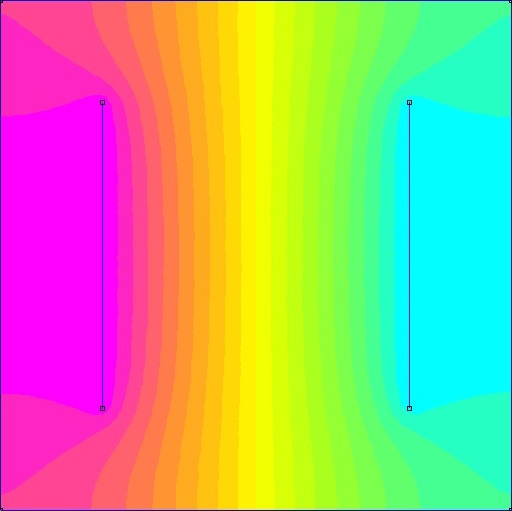
\includegraphics[width=\textwidth]{data/RandGross}
		\caption{Berandung durch Käfig}
		\label{fig:KäfigRand}
	\end{subfigure}
	\caption{Aufbau und Feldlinien des Kondensators}
\end{figure}

Vergleich man nun den Plot \ref{fig:kleinRand} mit \ref{fig:KäfigRand}, so wird eindeutig, dass die Feldlinien in Abbildung \ref{fig:kleinRand} senkrecht zu den beiden Flächen stehen. Berandet man den Kondensator durch einen Käfig, so werden auch die nicht senkrecht verlaufenden Feldlinien beachtet. In beiden Fällen entsteht ein homogenes Feld. Auch bei der Kapazität lassen sich unterschiedliche Werte ablesen. Während der Kondensator \ref{fig:kleinRand} eine Kapazität von \SI{2,6562}{\pico\farad} hat, liegt die Kapazität von Kondensator \ref{fig:KäfigRand} bei \SI{3,9773}{\pico\farad} \newpage
Zusätzlich soll verglichen werden, wie sich verschiedene Randbedingungen auf das entstehende elektrische Feld auswirken. Hierzu wurden dem Rand verschiedene Werte zugewiesen. Zunächst in Abbildung \ref{fig:0V} eine Spannung von \SI{0}{\volt}, dann in Abbildung \ref{fig:0,5V} \SI{0,5}{\volt} und schließlich eine Spannung von \SI{1}{\volt} in Abbildung \ref{fig:1V}. Es gilt die Selbe Skala, die in \ref{fig:Skala} zu sehen ist.

\begin{figure}[h]
	\begin{subfigure}[c]{0.32\textwidth}
		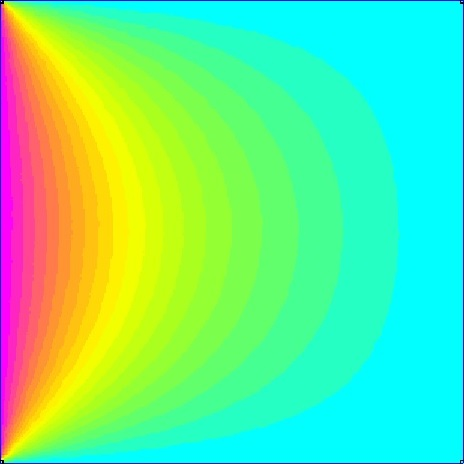
\includegraphics[width=\textwidth]{data/0VRandbedingung}
		\caption{Rand mit 0V Spannung}
		\label{fig:0V}
	\end{subfigure}
	\begin{subfigure}[c]{0.32\textwidth}
		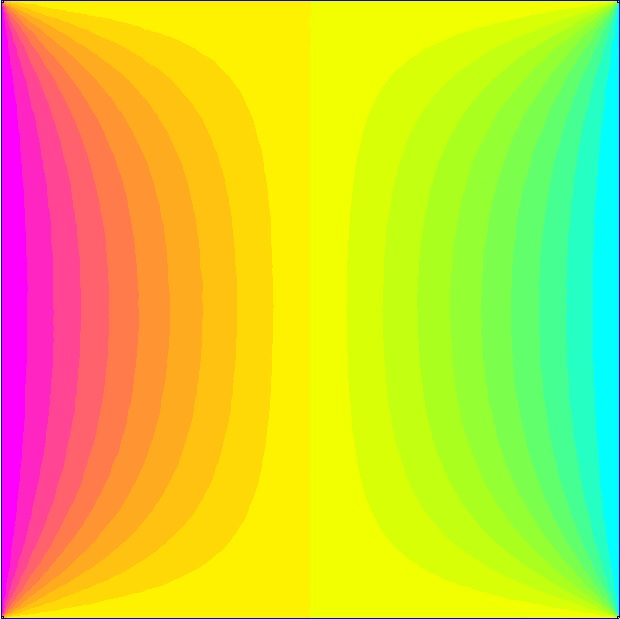
\includegraphics[width=\textwidth]{data/0,5VRandbedingung}
		\caption{Rand mit 0,5V Spannung}
		\label{fig:0,5V}
	\end{subfigure}
	\begin{subfigure}[c]{0.32\textwidth}
		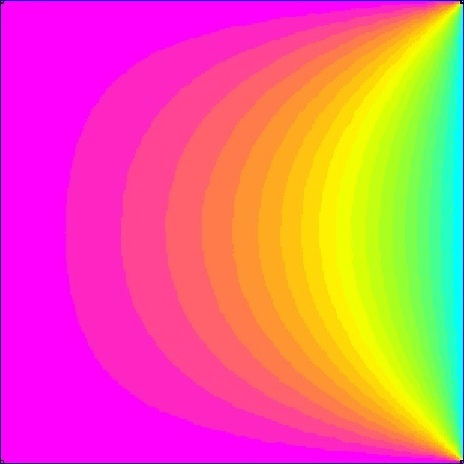
\includegraphics[width=\textwidth]{data/1VRandbedingung}
		\caption{Rand mit 1V Spannung}
		\label{fig:1V}
	\end{subfigure}
	\caption{Darstellung unterschiedlicher Randbedingungen}
\end{figure}

Da nun unterschiedliche Randbedingungen herrschen, entstehen auch Feldlinien zwischen den Kondensatorplatten und dem Rand. Es ergeben sich nicht nur unterschiedliche Feldlinien, sondern auch verschiedene Kapazitäten an den beiden Platten. 
\vspace*{1.5cm}

\begin{table}[h]
	\centering
	\begin{tabular}[h]{c|c c}
		Spannung am Rand & Kapazität linke Kondensatorplatte & Kapazität rechte Kondensatorplatte \\
		\hline
		\SI{0}{\volt} &  \SI{22,1405}{\pico\farad} & \SI{-0,5861}{\pico\farad} \\
		\SI{0,5}{\volt} & \SI{11,3633}{\pico\farad} & \SI{-11,3633}{\pico\farad} \\
		\SI{1}{\volt} &  \SI{0,5861}{\pico\farad} & \SI{-22,1405}{\pico\farad}
	\end{tabular}
\end{table}
\vspace*{1.5cm}
Die Feldlinien werden offensichtlich durch die anliegende Spannung am Rand beeinflusst und damit auch die Kapazität des Kondensators.
\\
\\
FEMM lässt sich nicht nur mit Hilfe von Octave starten, sondern es besteht auch die Möglichkeit eine OctaveFEMM Routine zu schreiben und damit ein Modell zu erstellen, sowie eine Simulation dieses Modells zu starten. In dem gegebenen Fall, soll eine Routine geschrieben werden, die zwei Parameter $a$ und $h$ entgegen nimmt, wobei $a$ die Kantenlänge und $h$ der Abstand der Platten ist. Aus diesen Informationen soll ein Kondensator erstellt und die berechnete Kapazität $C$ zurückgeliefert werden. Der Quellcode befindet sich im Anhang. \\ 
\newpage
Zunächst wird in Zeile 7 bis 9 FEMM geöffnet und definiert um welche Art von Problem es sich handelt. Zusätzlich werden einige Einstellungen getroffen, wie die Einheit der Variablen, die Tiefe des Modells und die Rechengenauigkeit. \\ 
In Zeile 10 bis 13 werden die verschiedenen Properties erzeugt, also die Randbedingungen (falls gewünscht), die Kondensatorplatten und das Dielektrikum. \\
Durch den Befehl in Zeile 16 wird daraufhin ein Rechteck, mit Hilfe der an die Methode übergebenen Parameter,  erstellt. Ein Blocklabel für das Dielektrikum wird in Zeile 19 erzeugt. Von Zeile 22 bis 38 werden nun die einzelnen Properties den richtigen Linien und Punkten zugewiesen.\\
Bevor die Simulation starten kann, muss das Projekt gespeichert werden. Danach wird die Analyse auf dieser Datei gestartet und die Lösung graphisch auf dem Bildschirm angezeigt.\\
Der zurückzuliefernde Parameter $C$ ergibt sich nun aus dem Ergebnis der Ladung geteilt durch die Spannung. Diese sind in einem liegenden Vektor mit zwei Spalten gespeichert. Die Ladung an zweiter und die Spannung an erster Stelle. 